\documentclass[]{tufte-handout}

% ams
\usepackage{amssymb,amsmath}

\usepackage{ifxetex,ifluatex}
\usepackage{fixltx2e} % provides \textsubscript
\ifnum 0\ifxetex 1\fi\ifluatex 1\fi=0 % if pdftex
  \usepackage[T1]{fontenc}
  \usepackage[utf8]{inputenc}
\else % if luatex or xelatex
  \makeatletter
  \@ifpackageloaded{fontspec}{}{\usepackage{fontspec}}
  \makeatother
  \defaultfontfeatures{Ligatures=TeX,Scale=MatchLowercase}
  \makeatletter
  \@ifpackageloaded{soul}{
     \renewcommand\allcapsspacing[1]{{\addfontfeature{LetterSpace=15}#1}}
     \renewcommand\smallcapsspacing[1]{{\addfontfeature{LetterSpace=10}#1}}
   }{}
  \makeatother

\fi

% graphix
\usepackage{graphicx}
\setkeys{Gin}{width=\linewidth,totalheight=\textheight,keepaspectratio}

% booktabs
\usepackage{booktabs}

% url
\usepackage{url}

% hyperref
\usepackage{hyperref}

% units.
\usepackage{units}


\setcounter{secnumdepth}{-1}

% citations

% pandoc syntax highlighting
\usepackage{color}
\usepackage{fancyvrb}
\newcommand{\VerbBar}{|}
\newcommand{\VERB}{\Verb[commandchars=\\\{\}]}
\DefineVerbatimEnvironment{Highlighting}{Verbatim}{commandchars=\\\{\}}
% Add ',fontsize=\small' for more characters per line
\newenvironment{Shaded}{}{}
\newcommand{\KeywordTok}[1]{\textcolor[rgb]{0.00,0.44,0.13}{\textbf{#1}}}
\newcommand{\DataTypeTok}[1]{\textcolor[rgb]{0.56,0.13,0.00}{#1}}
\newcommand{\DecValTok}[1]{\textcolor[rgb]{0.25,0.63,0.44}{#1}}
\newcommand{\BaseNTok}[1]{\textcolor[rgb]{0.25,0.63,0.44}{#1}}
\newcommand{\FloatTok}[1]{\textcolor[rgb]{0.25,0.63,0.44}{#1}}
\newcommand{\ConstantTok}[1]{\textcolor[rgb]{0.53,0.00,0.00}{#1}}
\newcommand{\CharTok}[1]{\textcolor[rgb]{0.25,0.44,0.63}{#1}}
\newcommand{\SpecialCharTok}[1]{\textcolor[rgb]{0.25,0.44,0.63}{#1}}
\newcommand{\StringTok}[1]{\textcolor[rgb]{0.25,0.44,0.63}{#1}}
\newcommand{\VerbatimStringTok}[1]{\textcolor[rgb]{0.25,0.44,0.63}{#1}}
\newcommand{\SpecialStringTok}[1]{\textcolor[rgb]{0.73,0.40,0.53}{#1}}
\newcommand{\ImportTok}[1]{#1}
\newcommand{\CommentTok}[1]{\textcolor[rgb]{0.38,0.63,0.69}{\textit{#1}}}
\newcommand{\DocumentationTok}[1]{\textcolor[rgb]{0.73,0.13,0.13}{\textit{#1}}}
\newcommand{\AnnotationTok}[1]{\textcolor[rgb]{0.38,0.63,0.69}{\textbf{\textit{#1}}}}
\newcommand{\CommentVarTok}[1]{\textcolor[rgb]{0.38,0.63,0.69}{\textbf{\textit{#1}}}}
\newcommand{\OtherTok}[1]{\textcolor[rgb]{0.00,0.44,0.13}{#1}}
\newcommand{\FunctionTok}[1]{\textcolor[rgb]{0.02,0.16,0.49}{#1}}
\newcommand{\VariableTok}[1]{\textcolor[rgb]{0.10,0.09,0.49}{#1}}
\newcommand{\ControlFlowTok}[1]{\textcolor[rgb]{0.00,0.44,0.13}{\textbf{#1}}}
\newcommand{\OperatorTok}[1]{\textcolor[rgb]{0.40,0.40,0.40}{#1}}
\newcommand{\BuiltInTok}[1]{#1}
\newcommand{\ExtensionTok}[1]{#1}
\newcommand{\PreprocessorTok}[1]{\textcolor[rgb]{0.74,0.48,0.00}{#1}}
\newcommand{\AttributeTok}[1]{\textcolor[rgb]{0.49,0.56,0.16}{#1}}
\newcommand{\RegionMarkerTok}[1]{#1}
\newcommand{\InformationTok}[1]{\textcolor[rgb]{0.38,0.63,0.69}{\textbf{\textit{#1}}}}
\newcommand{\WarningTok}[1]{\textcolor[rgb]{0.38,0.63,0.69}{\textbf{\textit{#1}}}}
\newcommand{\AlertTok}[1]{\textcolor[rgb]{1.00,0.00,0.00}{\textbf{#1}}}
\newcommand{\ErrorTok}[1]{\textcolor[rgb]{1.00,0.00,0.00}{\textbf{#1}}}
\newcommand{\NormalTok}[1]{#1}

% longtable

% multiplecol
\usepackage{multicol}

% strikeout
\usepackage[normalem]{ulem}

% morefloats
\usepackage{morefloats}


% tightlist macro required by pandoc >= 1.14
\providecommand{\tightlist}{%
  \setlength{\itemsep}{0pt}\setlength{\parskip}{0pt}}

% title / author / date
\title{Data collection and summarization}
\author{Patrick Ding}
\date{8/28/2018}


\begin{document}

\maketitle




\section{Topic Overview}\label{topic-overview}

\begin{itemize}
\tightlist
\item
  Populations and samples
\item
  Frequency distributions
\item
  Histograms
\item
  Mean, median, variance and standard deviation
\item
  Quartiles, interquartile range
\item
  Boxplots
\end{itemize}

\section{What is Statistics?}\label{what-is-statistics}

\begin{itemize}
\item
  Statistics: the science of collecting, classifying, and interpreting
  data.
\item
  Anticipated learning outcomes:

  \begin{itemize}
  \tightlist
  \item
    appreciate and apply basic statistical methods in an everyday life
    setting
  \item
    appreciate and apply basic statistical methods in their scientific
    field
  \end{itemize}
\end{itemize}

\section{Where will Statistics be
used?}\label{where-will-statistics-be-used}

\begin{itemize}
\tightlist
\item
  Everyday life

  \begin{itemize}
  \tightlist
  \item
    Proper application of general probabilities
  \item
    How election results are presented
  \item
    Commercial claims (clinical trials vs.~outliers)
  \end{itemize}
\item
  Industry applications

  \begin{itemize}
  \tightlist
  \item
    Google web searches
  \item
    Netflix user recommendations
  \item
    Pharmaceutical drug development
  \item
    Sports analytics
  \item
    Modeling global climate change
  \item
    Credit card fraud detection
  \item
    Biomarkers and disease detection
  \item
    Criminal justice
  \end{itemize}
\end{itemize}

\section{Collecting data}\label{collecting-data}

\begin{itemize}
\item
  \textbf{Observational study}: Observe a group and measure quantities
  of interest. This is passive data collection in that one does not
  attempt to influence the group. The purpose of the study is to
  describe the group.
\item
  \textbf{Experiment}: Deliberately impose treatments on groups in order
  to observe responses. The purpose is to study whether the treatments
  cause a change in the responses.
\end{itemize}

\section{Observational Study}\label{observational-study}

\subsection{Definitions}\label{definitions}

\begin{enumerate}
\def\labelenumi{\arabic{enumi}.}
\item
  \textbf{Population}: The entire group of interest
\item
  \textbf{Sample}: A part of the population selected to draw conclusions
  about the entire population
\item
  \textbf{Census}: A sample that attempts to include the entire
  population
\item
  \textbf{Parameter}: A concept that describes the population
\item
  \textbf{Statistic}: A number produced from a sample that estimates a
  population parameter
\end{enumerate}

\section{Experiment}\label{experiment}

\begin{enumerate}
\def\labelenumi{\arabic{enumi}.}
\item
  \textbf{Experimental Group}: A collection of experimental units
  subjected to a difference in treatment, imposed by the experimenter.
\item
  \textbf{Control Group}: A collection of experimental units subjected
  to the same conditions as those in an experimental group except that
  no treatment is imposed.
\end{enumerate}

This design helps control for potential confounding effects.

\section{Cereal Data}\label{cereal-data}

\begin{figure}
\centering
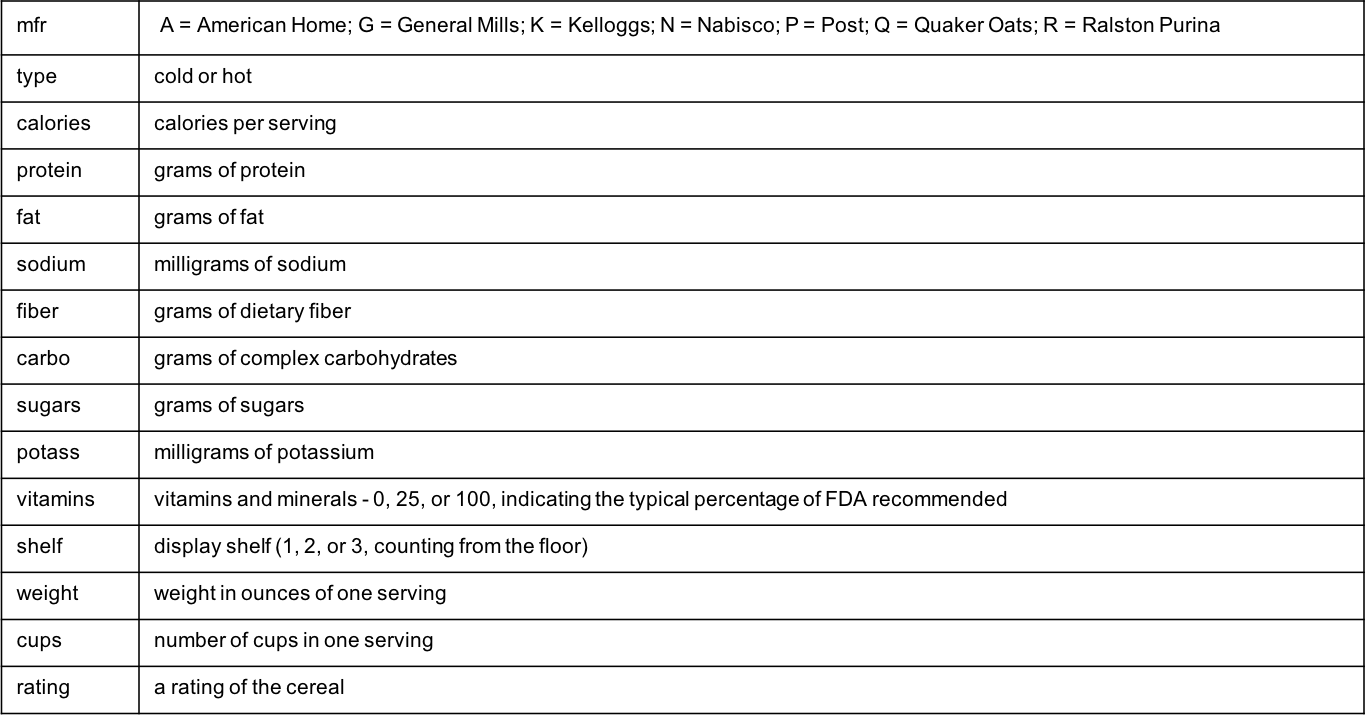
\includegraphics{UScereal.png}
\caption{US cereal data}
\end{figure}

\section{Summarizing single categorical
variable}\label{summarizing-single-categorical-variable}

\begin{itemize}
\tightlist
\item
  \textbf{Frequency} - number of times the value occurs in the data
\item
  \textbf{Relative frequency} - proportion of the data with the value
\end{itemize}

\section{Summarizing single categorical
variable}\label{summarizing-single-categorical-variable-1}

\begin{verbatim}
## mfr
##  G  K  N  P  Q  R 
## 22 21  3  9  5  5 
## mfr
##          G          K          N          P 
## 0.33846154 0.32307692 0.04615385 0.13846154 
##          Q          R 
## 0.07692308 0.07692308
\end{verbatim}

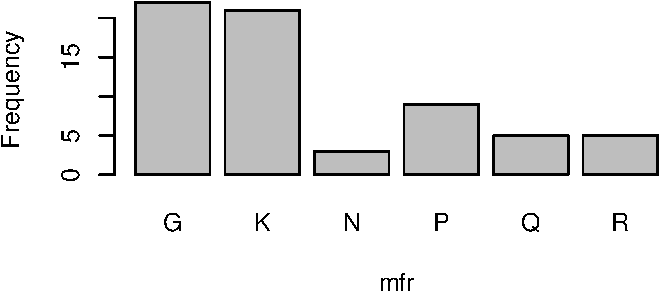
\includegraphics{data_collection_summary_files/figure-latex/unnamed-chunk-1-1}

\section{R script for histograms of state
data}\label{r-script-for-histograms-of-state-data}

\begin{Shaded}
\begin{Highlighting}[]
\KeywordTok{summary}\NormalTok{(USArrests)}
\end{Highlighting}
\end{Shaded}

\begin{verbatim}
##      Murder          Assault     
##  Min.   : 0.800   Min.   : 45.0  
##  1st Qu.: 4.075   1st Qu.:109.0  
##  Median : 7.250   Median :159.0  
##  Mean   : 7.788   Mean   :170.8  
##  3rd Qu.:11.250   3rd Qu.:249.0  
##  Max.   :17.400   Max.   :337.0  
##     UrbanPop          Rape      
##  Min.   :32.00   Min.   : 7.30  
##  1st Qu.:54.50   1st Qu.:15.07  
##  Median :66.00   Median :20.10  
##  Mean   :65.54   Mean   :21.23  
##  3rd Qu.:77.75   3rd Qu.:26.18  
##  Max.   :91.00   Max.   :46.00
\end{verbatim}

\begin{Shaded}
\begin{Highlighting}[]
\KeywordTok{par}\NormalTok{(}\DataTypeTok{mfrow =} \KeywordTok{c}\NormalTok{(}\DecValTok{1}\NormalTok{, }\DecValTok{2}\NormalTok{))}
\KeywordTok{hist}\NormalTok{(USArrests}\OperatorTok{$}\NormalTok{Murder, }\DataTypeTok{main =} \StringTok{"Murder"}\NormalTok{)}
\KeywordTok{hist}\NormalTok{(USArrests}\OperatorTok{$}\NormalTok{UrbanPop, }\DataTypeTok{main =} \StringTok{"Urban Population"}\NormalTok{)}
\end{Highlighting}
\end{Shaded}

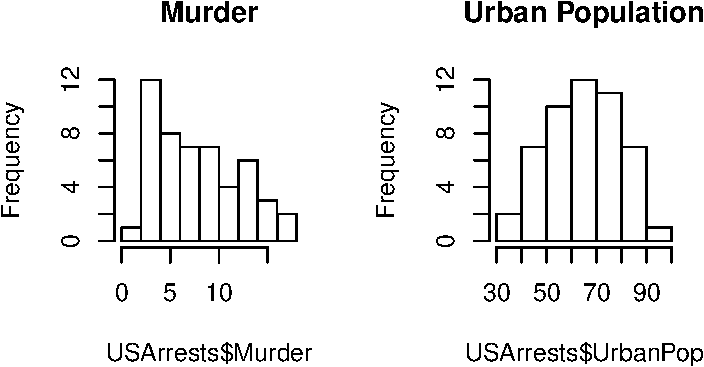
\includegraphics{data_collection_summary_files/figure-latex/unnamed-chunk-2-1}

\section{Summary statistics for quantitative
data}\label{summary-statistics-for-quantitative-data}

\subsection{Measures of central
tendency}\label{measures-of-central-tendency}

\begin{itemize}
\item
  The \textbf{sample median} is the middle observation if the values are
  arranged in increasing order.
\item
  The \textbf{sample mean} of n observations is the average, the sum of
  the values divided by n:
\end{itemize}

\begin{align}
\bar{x} = \frac{1}{n}\sum_{i=1}^n x_i
\end{align}



\end{document}
